% arguelles v2.3.0
% author: Michele Piazzai
% contact: michele.piazzai@uc3m.es
% license: MIT

\documentclass[compress,12pt]{beamer}
\usepackage{hyperref}
\hypersetup{pdfpagemode=FullScreen}
\usepackage{tikz}
\usepackage{nicefrac}
\usepackage[round]{natbib}

\graphicspath{{figs}}
\newcommand{\emoji}[1]{\includegraphics[height=\fontcharht\font`\B]{emojis/#1.png}}

\newcommand{\xmark}{%
\tikz[scale=0.15] {
      \draw[line width=0.7,line cap=round] (0,0) to [bend left=6] (1,1);
      \draw[line width=0.7,line cap=round] (0.2,0.95) to [bend right=3] (0.8,0.05);
}}
\newcommand{\cmark}{%
\tikz[scale=0.15] {
      \draw[line width=0.7,line cap=round] (0.25,0) to [bend left=10] (1,1);
      \draw[line width=0.8,line cap=round] (0,0.35) to [bend right=1] (0.23,0);
}}

\usetheme{Arguelles}


\addtobeamertemplate{navigation symbols}{}{%
      \usebeamerfont{footline}%
      \usebeamercolor[fg]{footline}%
      \hspace{1em}%
      \vspace{1em}%
      \insertframenumber/\inserttotalframenumber
}

\title{Explainable AI is Dead, Long Live Explainable AI!}
\subtitle{Hypothesis-driven Decision Support using Evaluative AI}
\event{Tim \cite{evaluative-ai} - Conference FAccT}
\date{}
\author{\tiny Charles Vin}
\institute{\tiny Sorbonne Université - 21216136}
% \email{charles.vin@outlook.fr}
% \homepage{charles.vin}
% \github{username}

\begin{document}

\frame[noframenumbering, plain]{\titlepage}

\Section{Introduction}
\begin{frame}
      \frametitle{Quick summary}
      Arg for a Paradigm Shift in XAI for Decision Support \\
      $\rightarrow$ Evaluative AI Concept \\
      Goals:
      \begin{itemize}
            \item Human-centered Approach.
            \item Going Beyond Recommendations.
            \item \textbf{Mitigating Over-Reliance}.
            \item Support for Hypothesis Evaluation.
            \item Machine-in-the-Loop Paradigm.
      \end{itemize}
\end{frame}

\subsection{Over/Under reliance}
\begin{frame}
      \frametitle{Over/Under-reliance}
      \framesubtitle{Definitions}
      \begin{itemize}
            \item \textbf{Over-reliance}: Decision makers accept a machine recommendations, even when it is wrong, but would be rejected if coming from a human. \begin{itemize}
                  \item \textit{The machine "must be right" because it's a machine}
            \end{itemize}
            \item \textbf{Under-reliance}: Machine outputs are consistently rejected, even when it is correct, but would be accepted if coming from a human. 
      \end{itemize}
      See \href{https://en.wikipedia.org/wiki/Automation_bias}{\textit{''Automation bias''}}
      $ \Rightarrow  $ Problems after deployement: \\ 
      AI systems ignored OR over-reliance related problems.
\end{frame}

\begin{frame}
      \frametitle{Over/Under-reliance}
      \framesubtitle{Causes}
      \begin{itemize}
            \item Over-reliance: lack of cognitive engagement.
            \item Under-reliance: Algorithmic aversion.
      \end{itemize}
      When adding current XAI tools for more explaination \\
      $ \Rightarrow $ Confirmation bias (called \textit{fixation} in the paper).
\end{frame}

\begin{frame}
      \frametitle{Over/Under-reliance}
      \framesubtitle{Solutions}
      \begin{enumerate}
            \item Cognitive forcing \begin{itemize}
                  \item Eg. forcing people to give a decision before seeing a recommendation.
                  \item Slightly mitigated overreliance, but not enought to lead to a statistically significant differences.
                  \item Least prefered method by participant : people not wanting to exert mental energy.
            \end{itemize}
            \item Changing the XAI framework \emoji{smirking-face} \emoji{thinking-face} \emoji{thought-balloon} \emoji{light-bulb}
      \end{enumerate}
\end{frame}

\begin{frame}
      \frametitle{How we make decisions?}
      In a simple way: 
      \begin{itemize}
            \item Identify options.
            \item Compare options.
            \item Choose an option.
      \end{itemize}
      In a less simple way: the 10 "cardinal decision issue" outlined by \cite{evidence-based-decision-management} \begin{itemize}
            \item Needs, mode, Investment, Options, Possibilities, Judgements, Value, Trade-offs, Acceptability, Implementation.
      \end{itemize}
\end{frame}

\begin{frame}
      \frametitle{What makes a good decisions support system?}
      \framesubtitle{Summed up}
      \begin{itemize}
            \item Options: Help to identify options, well as help to narrow down the list of feasible or realistic options.
            \item Judgement \& Possibilities: Help to judge which outcomes are most likely and what will be the positive and negative impacts.
            \item Trade-offs: Help to make trade-offs on the above criteria for each options.
            \item Understandable: Help to understand how and why the tools works as it does, and when it fails.
      \end{itemize}
\end{frame}


\section{Current XAI}

\begin{frame}[standout]
      \centering\large
      Does current decision support align with those criteria?
\end{frame}

\begin{frame}
      \frametitle{Giving recommendations with no explanatory information}
      \begin{columns}[T] % align columns
            \begin{column}{.75\textwidth}
                  \begin{figure}[htbp]
                        \centering
                        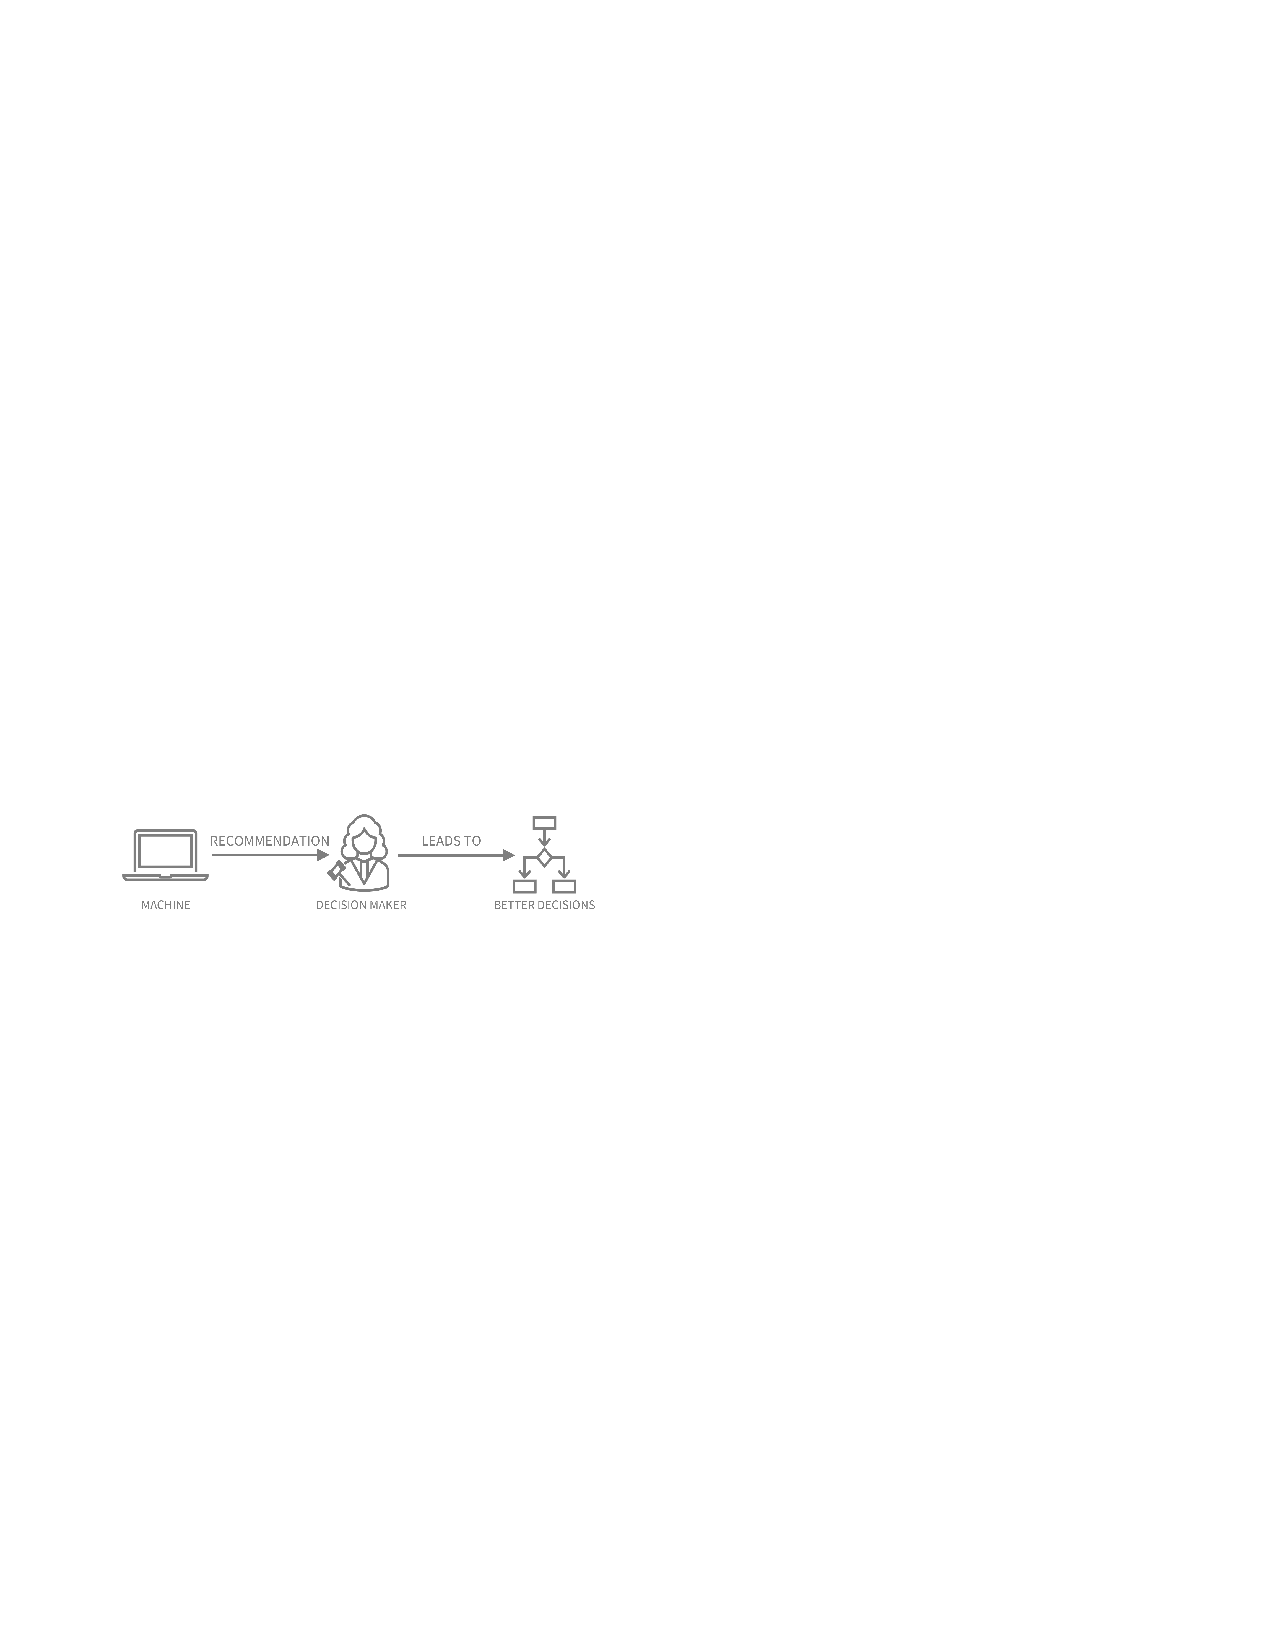
\includegraphics[width=.9\textwidth]{fig3.pdf}
                        \caption{ A model of giving recommendations for decision support.}
                  \end{figure}
                  \begin{itemize}
                        \item [] Decision makers can carefully consider recommendations.
                        \item [$\rightarrow$] Leading to better decisions. 
                        \item [\xmark] empirical evidence suggests this is not the case.
                  \end{itemize}
            \end{column}%
            \hfill%
            \begin{column}{.295\textwidth}
                  \begin{itemize}
                        \item[\xmark] Options
                        \item[$\nicefrac{1}{n}$] Possibilities \& Judgement
                        \item[\xmark] Trade-offs
                        \item[\xmark] Understandable
                  \end{itemize}
            \end{column}%
      \end{columns}
\end{frame}

\begin{frame}
      \frametitle{Giving recommendations with explanatory information}
      \begin{columns}[T] % align columns
            \begin{column}{.75\textwidth}
                  \begin{figure}[htbp]
                        \centering
                        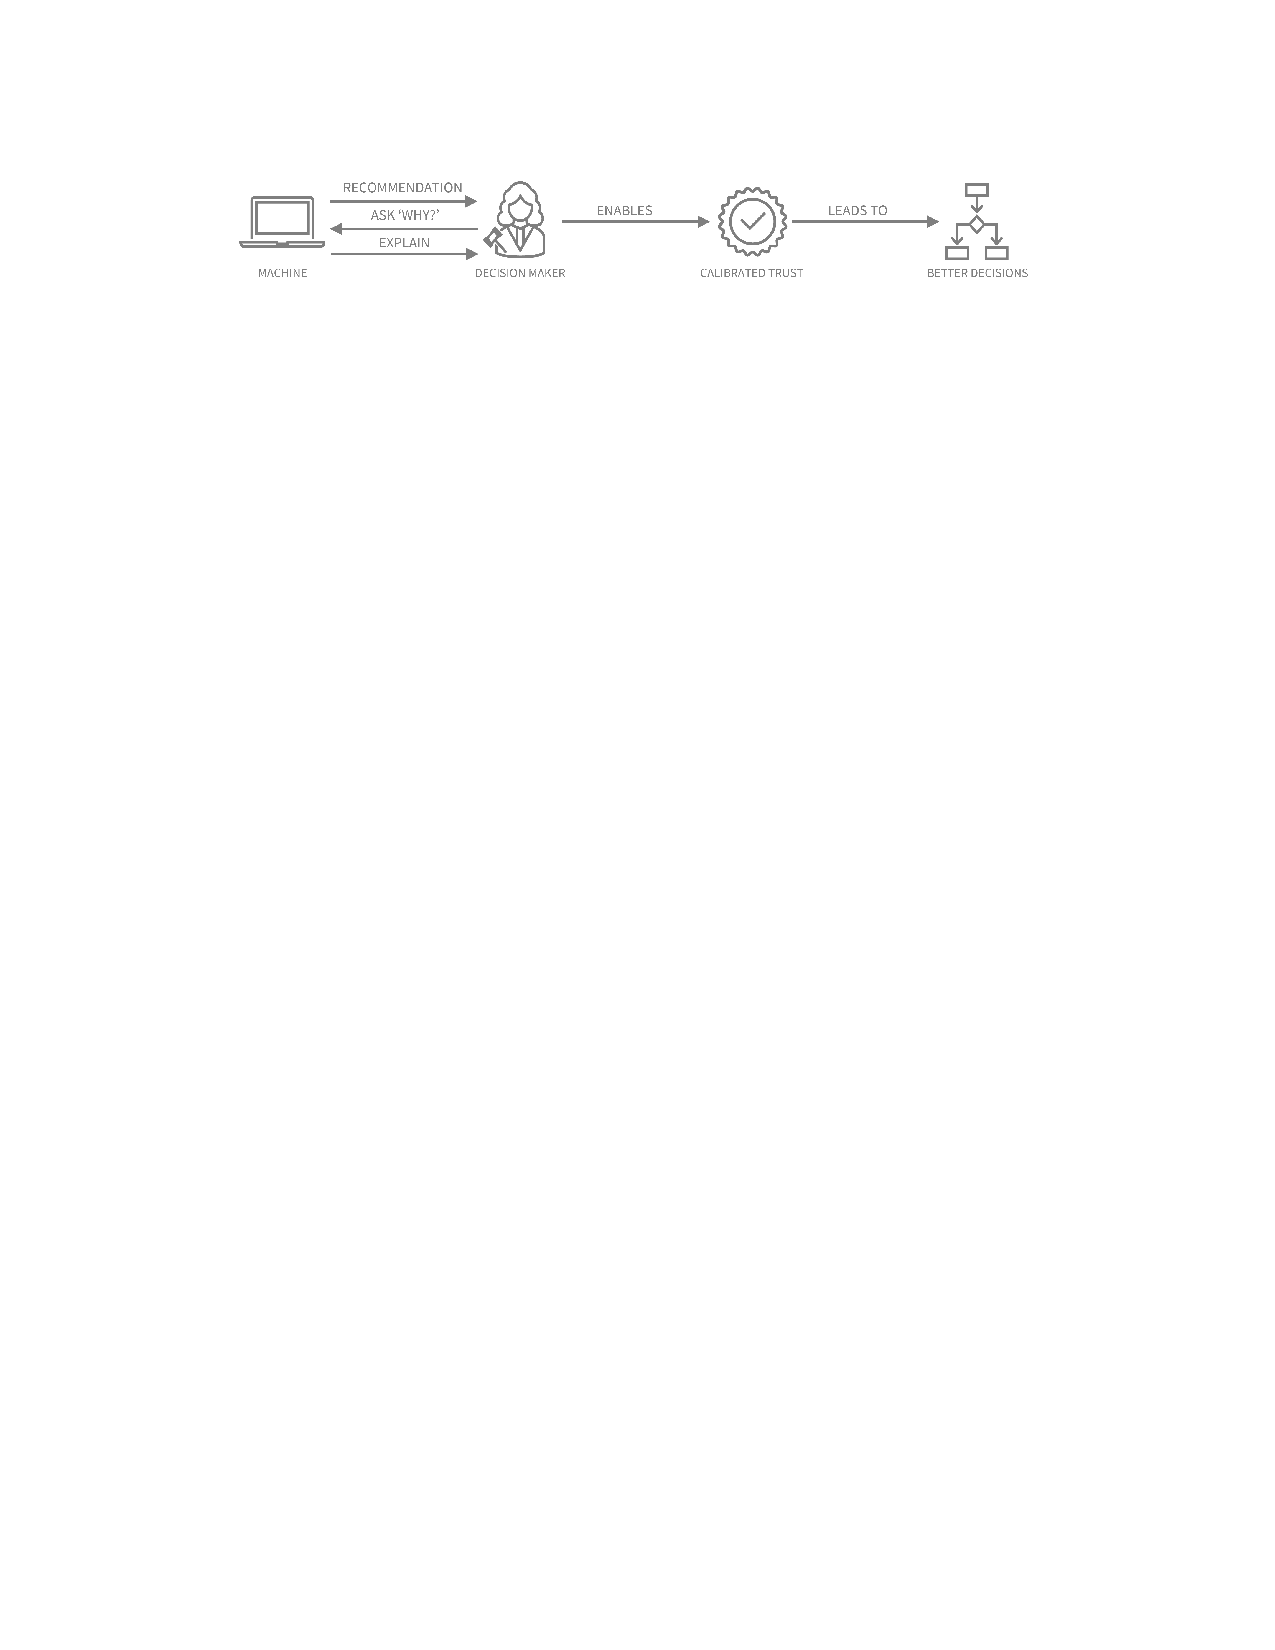
\includegraphics[width=.9\textwidth]{fig4.pdf}
                        \caption{A model of XAI for decision support.}
                  \end{figure}
                  \begin{itemize}
                        \item [] Giving reasons or explanations for decisions.
                        \item [$\rightarrow$] Mitigates the problem of distrust.
                        \item [$\rightarrow$] Leading to better decisions.
                        \item [\xmark] Empirical evidence suggests people do not pay careful attention to the reasons/explanations.
                  \end{itemize}
            \end{column}%
            \hfill%
            \begin{column}{.295\textwidth}
                  \begin{itemize}
                        \item[\xmark] Options
                        \item[$\nicefrac{1}{n}$] Possibilities \& Judgement
                        \item[\cmark/\xmark] Trade-offs
                        \item[\cmark] Understandable
                  \end{itemize}
            \end{column}%
      \end{columns}
\end{frame}

\begin{frame}
      \frametitle{Giving recommendations with cognitive forcing}
      \begin{columns}[T] % align columns
            \begin{column}{.705\textwidth}
                  \begin{figure}[htbp]
                        \centering
                        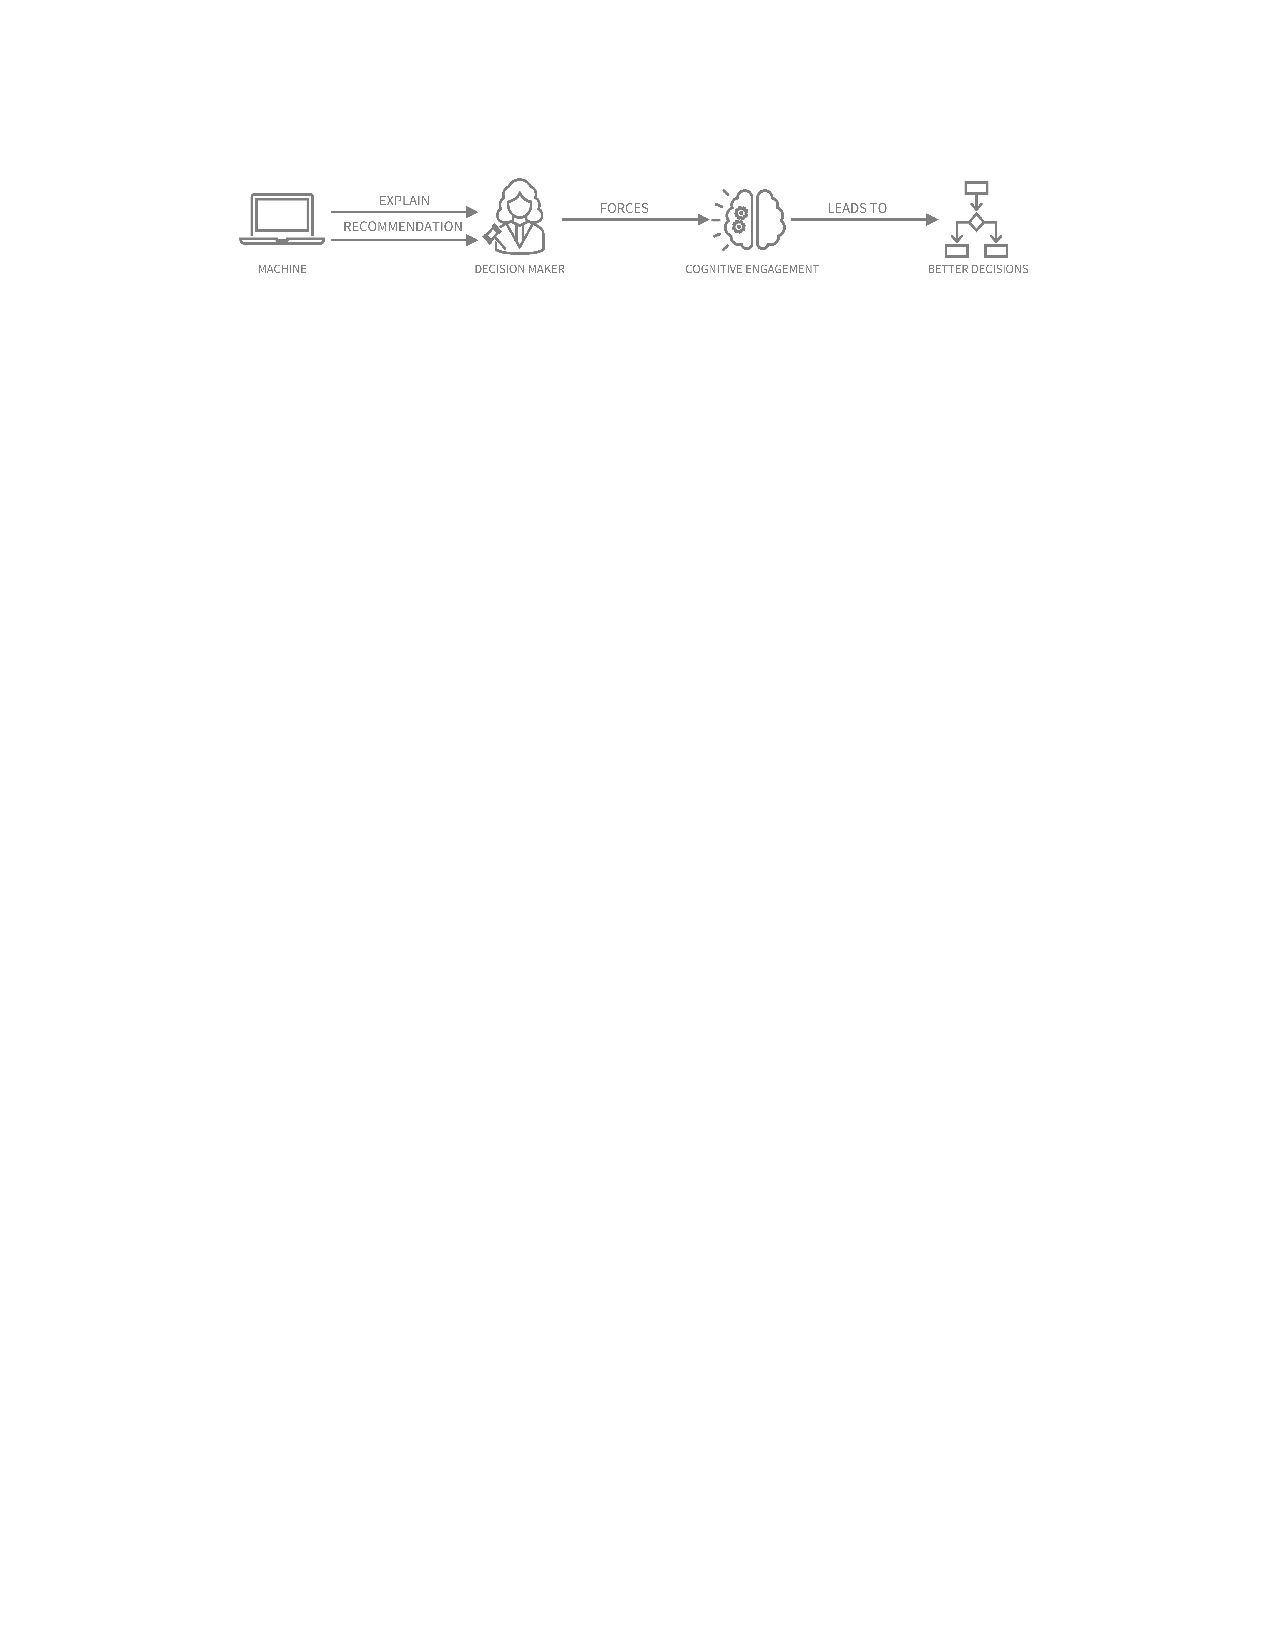
\includegraphics[width=.9\textwidth]{fig5.pdf}
                        \caption{A model of cognitive forcing.}
                  \end{figure}
                  \begin{itemize}
                        \item [] Withholding recommendations \& giving an explanation.
                        \item [$\rightarrow$] Forces people to engage.
                        \item [$\rightarrow$] Limit over-reliance.
                        \item [$\rightarrow$] Better decisions.
                        \item [\xmark] Still a ''recommend and defend'' approach.
                        \item [\xmark] Least prefered method by participants.
                  \end{itemize}
            \end{column}%
            \hfill%
            \begin{column}{.295\textwidth}
                  \begin{itemize}
                        \item[\cmark/\xmark] Options
                        \item[$\nicefrac{1}{n}$] Possibilities \& Judgement
                        \item[\cmark/\xmark] Trade-offs
                        \item[\cmark] Understandable
                  \end{itemize}
            \end{column}%
      \end{columns}
\end{frame}

\section{Evalative AI}
\begin{frame}
      \frametitle{The evaluative AI framework}
      \begin{columns}[T] % align columns
            \begin{column}{.5\textwidth}
                  \begin{figure}[htbp]
                        \centering
                        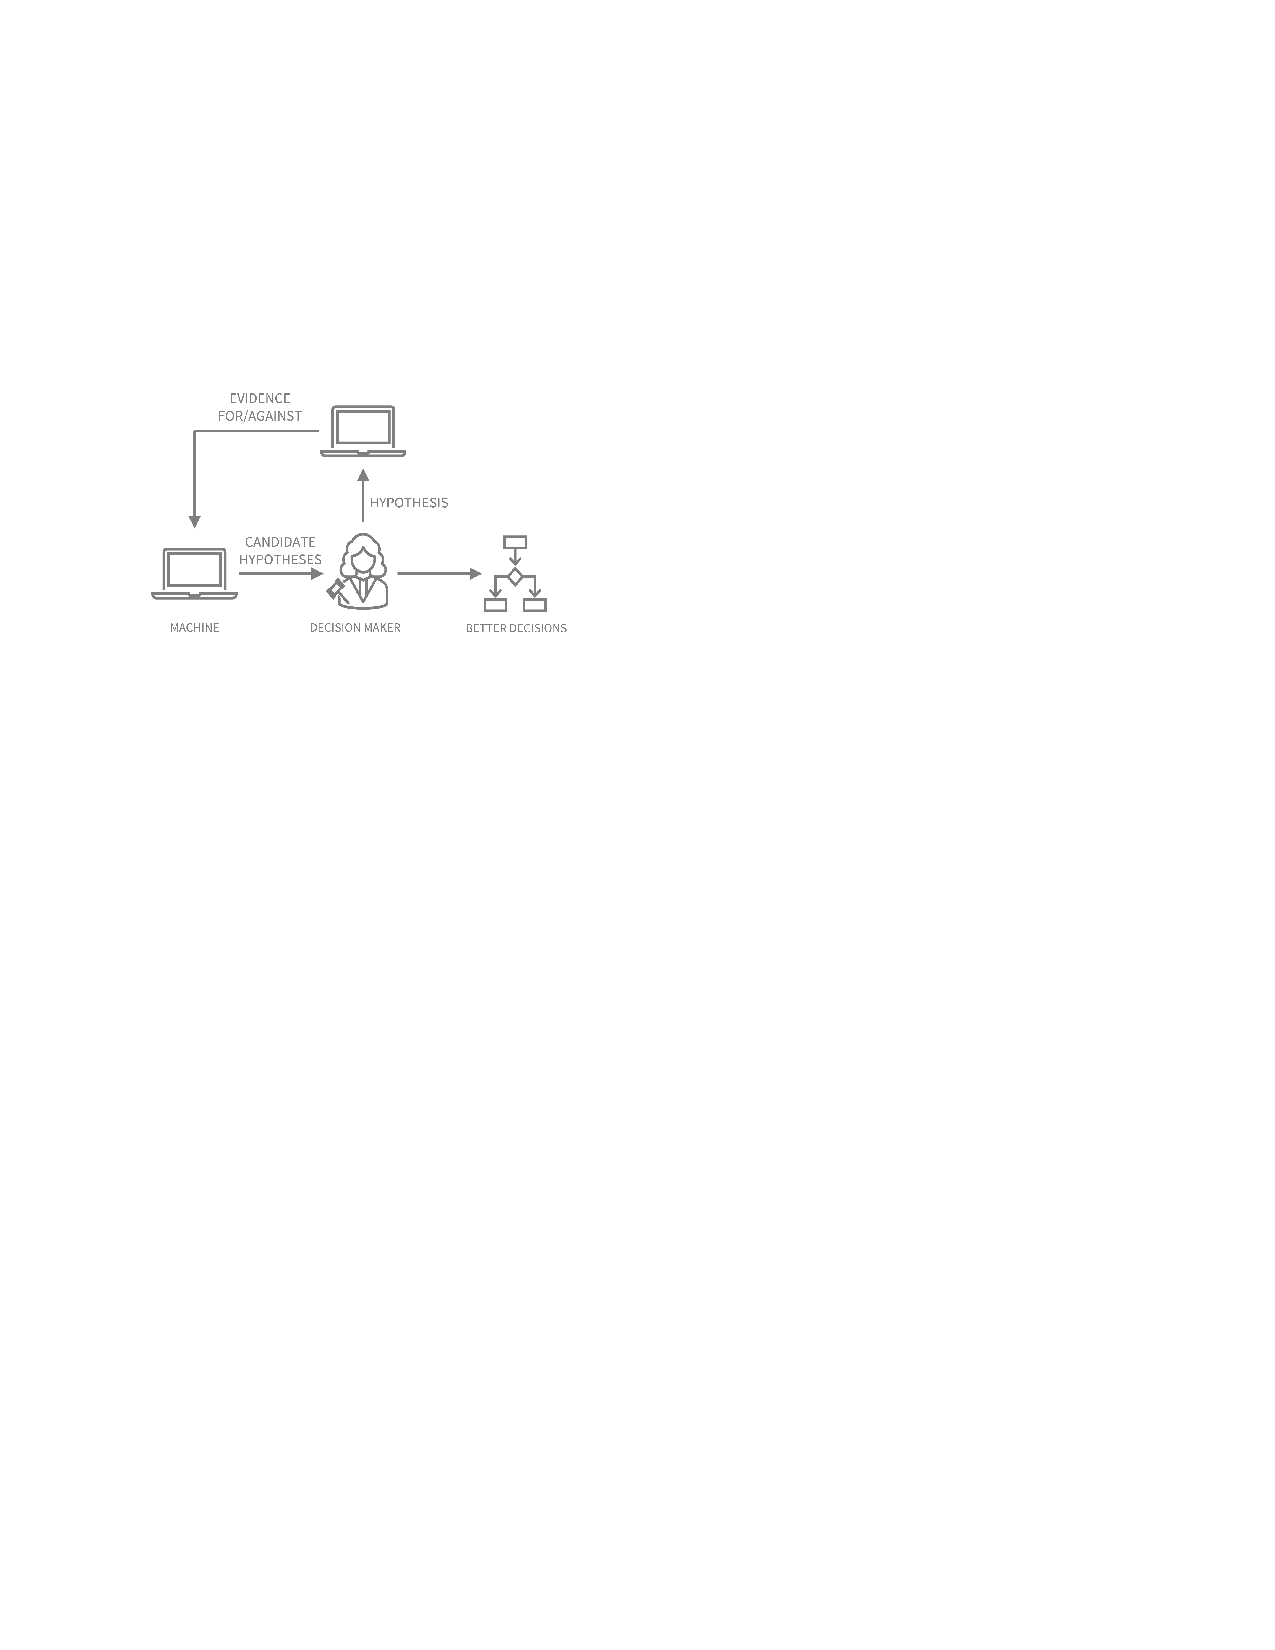
\includegraphics[width=\textwidth]{fig6.pdf}
                        \caption{A model of Evaluative AI.}
                  \end{figure}
            \end{column}%
            \hfill%
            \begin{column}{.5\textwidth}
                  \begin{itemize}
                        \item Align with decision making processes.
                        \item Keep the decision maker in control.
                        \item Ask users to rely on evidence instead of recommendations.
                  \end{itemize}
            \end{column}%
      \end{columns}
\end{frame}
\begin{frame}
      \frametitle{The evaluative AI framework}
      \framesubtitle{Exemple}
      \begin{columns}[T] % align columns
            \begin{column}{.705\textwidth}
                  \begin{figure}[htbp]
                        \centering
                        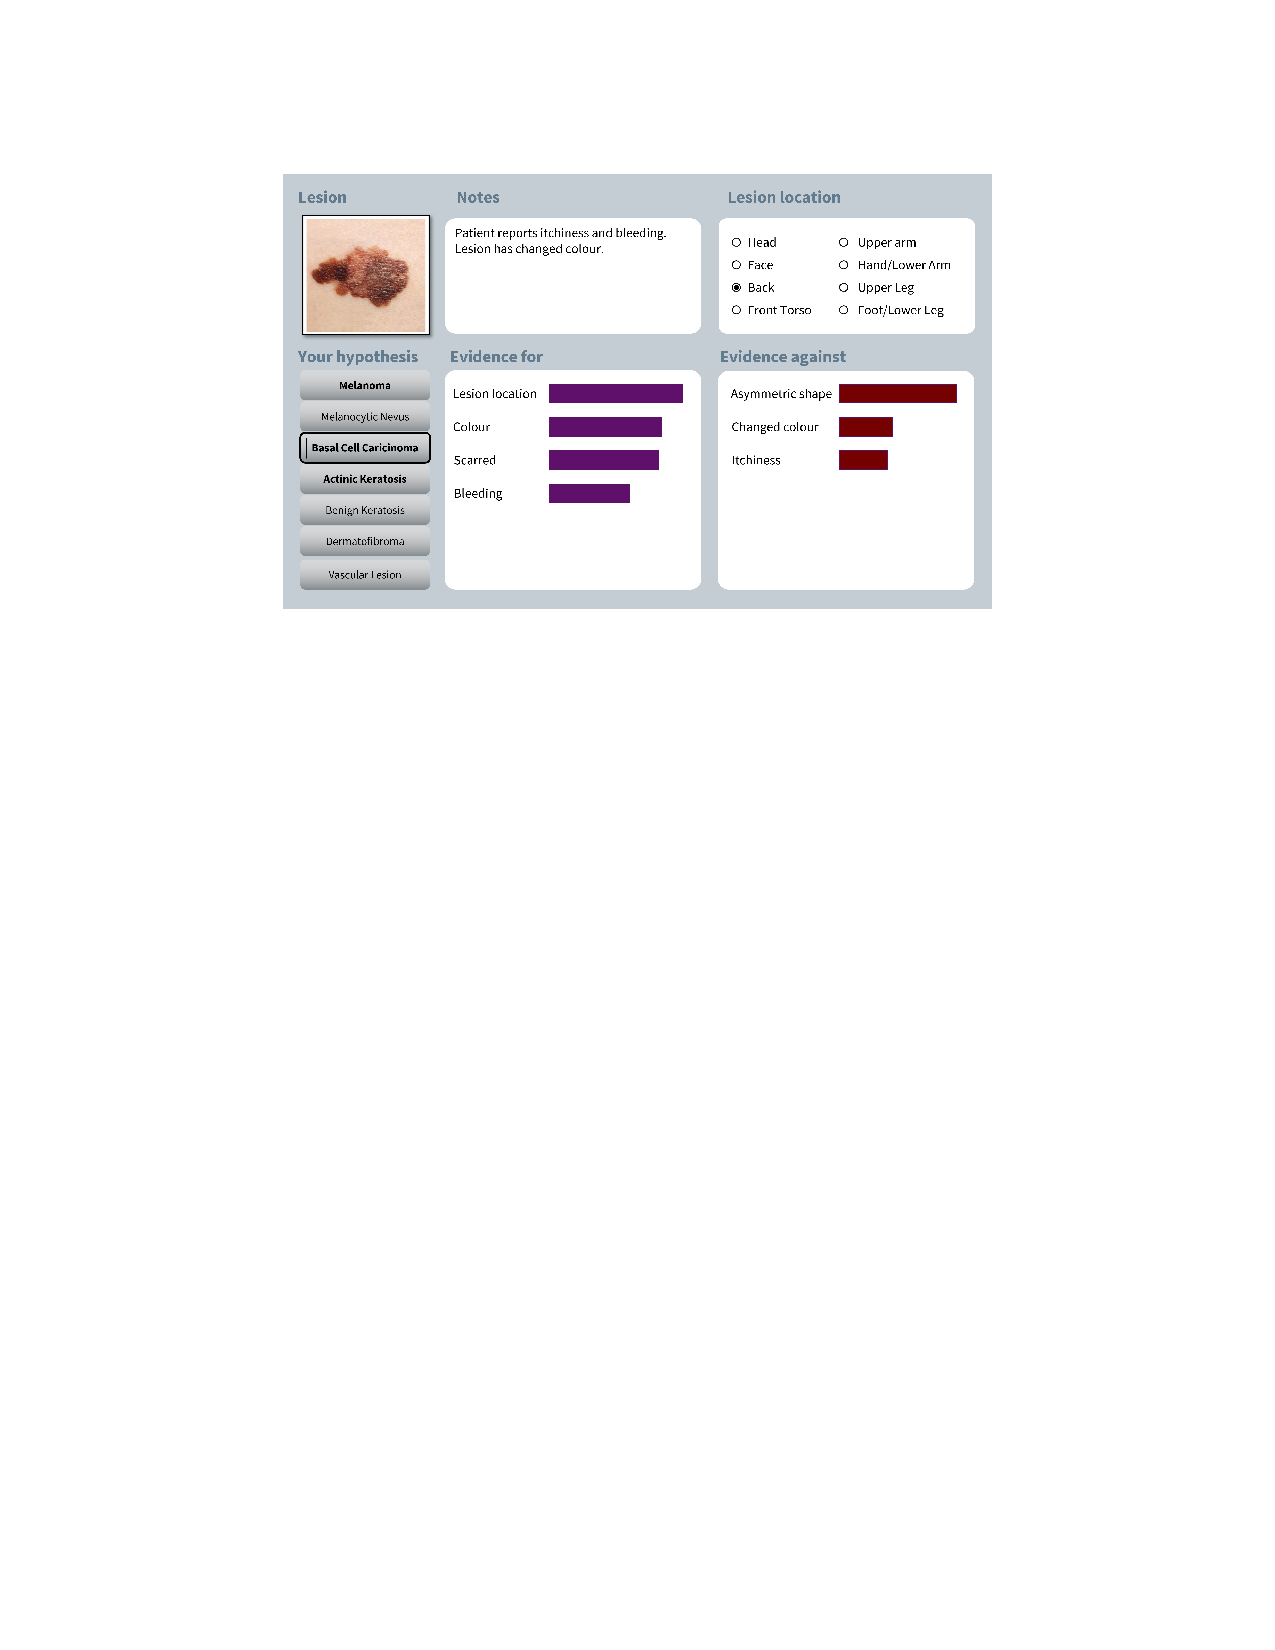
\includegraphics[width=\textwidth]{exmp.pdf}
                        \caption{A simple prototype of a diagnostic interface using evaluative AI.}
                  \end{figure}
            \end{column}%
            \hfill%
            \begin{column}{.295\textwidth}
                  \begin{itemize}
                        \item[\cmark] Options
                        \item[\cmark] Possibilities \& Judgement
                        \item[\cmark] Trade-offs
                        \item[\cmark] Understandable
                  \end{itemize}
            \end{column}%
      \end{columns}
\end{frame}
\begin{frame}
      \frametitle{The evaluative AI framework}
      \framesubtitle{Zoom on properties}
      \begin{itemize}
            \item[\cmark] Options \begin{itemize}
                  \item Show the most likely options (with or without probabilities).
                  \item [$\rightarrow$] Not a single recommendation.
            \end{itemize}
            \item[\cmark] Possibilities \& Judgement \begin{itemize}
                  \item The machine provide feedback on humain jugement only.
            \end{itemize}
            \item[\cmark] Trade-offs \begin{itemize}
                  \item Offer real trade-offs between \textit{any} set of two options.
                  \item Evaluative AI provides evidence both for and against each option, irrelevant of the judged likelihood of that option.
                  \item [$\rightarrow$] \textit{Option awareness} in the literature.
            \end{itemize}
      \end{itemize}
\end{frame}

\begin{frame}
      \frametitle{Limitation}
      \framesubtitle{mentionned by the author}
      \begin{itemize}
            \item Why would people pay attention to evidence this time? \begin{itemize}
                  \item [$\rightarrow$] Evaluative AI \begin{itemize}
                        \item Better control.
                        \item Process built on the way we makes naturally decision \\
                        $\rightarrow$ people would naturally follow \\
                        $ \neq  $ Contrary to recommendation-driven approches.
                  \end{itemize}
                  \item [\xmark] Proof ?
            \end{itemize}
            \item Cognitive load remain a problem \begin{itemize}
                  \item [$\rightarrow$] Evaluative AI still reduce the quantity of information the decision maker.needs (only revelant information are presented)
                  \item [\xmark] Still the less prefered solution by decision makers.
            \end{itemize}
      \end{itemize}
\end{frame}

\begin{frame}
      \frametitle{Limitation}
      \framesubtitle{from my pov}
      \begin{itemize}
            \item Vague criterias.
            \item More introduction around automation bias needed, was this litterature explored ?
      \end{itemize}
\end{frame}
\begin{frame}
      \frametitle{Strength}
      \framesubtitle{from my pov}
      \begin{itemize}
            \item Solve a real problem. 
            \item Propose something to move forward.
            \item Give a precise research agenda.
      \end{itemize}
\end{frame}

\End
\begin{frame}[standout]
      \centering\large
      Conclusion
\end{frame}
\begin{frame}[plain,standout]
      \centering\LARGE
      Thank you
\end{frame}

\begin{frame}
      \frametitle{Bibliography}
      \scriptsize{
            \bibliographystyle{plainnat}
            \bibliography{bib}
            \href{https://github.com/piazzai/arguelles}{Beamer template from here \faGithub} \\
      }
\end{frame}

\section{Bonus slides}
\begin{frame}
      \frametitle{The evaluative AI framework \\ \normalsize Differences with cognitive forcing}
      \begin{itemize}
            \item \textbf{Control} Permit to explore hypothesis, not a single recommendation.
            \item [$\rightarrow$] Built on the way we makes decision (identify, compare, choose).
      \end{itemize}
\end{frame}
\begin{frame}
      \frametitle{Long live XAI}
      \begin{itemize}
            \item Evaluative AI is designed only toward decision making, $ \text{Evaluative AI} \subset \text{XAI} $.
            \item XAI is still needed and more adapted to many situation (eg. making decision at scale).
            \item Recommendation based models : base of any XAI techniques.
            \item Many existing XAI tools are already adapted to Evaluative AI \begin{itemize}
                  \item Constrastive explanation.
                  \item Feature importance (eg. SHAP).
            \end{itemize}
      \end{itemize}
\end{frame}


\end{document}